%\section{Pipelines Network Analysis}
%The prior chapter introduced the non-linear system that results from the analysis of the pipeline network.  
%This chapter continues the effort and produces a workable \textbf{R} script that can compute flows and heads given just the node-arc incidence matrix, and pipe properties.
%
%Recall from the prior chapter the non-linear system to be solved is
%\begin{displaymath}
%\mathbf{A(x)} \cdot \mathbf{x} = \mathbf{b}
%  \end{displaymath}
%  
%  which would look like
%  
%\begin{gather}
%\begin{pmatrix}
%~1&-1 & 0  & -1 & 0 & 0 & 0 & 0 & 0 &0 \\
%0&~1 & -1  & 0 & 0 &~1 & 0 & 0 & 0 &0 \\
%0& 0 & 0 &~1 & -1 & -1 & 0 & 0 & 0 &0 \\
%0& 0 &~1  & 0 &~1 & 0 & 0  & 0 & 0 &0 \\
%\hline
%-L_1& 0& 0 & 0 & 0 & 0 & -1 & 0 & 0 &0 \\
%0& -L_2& 0 & 0 & 0 & 0&~1 & -1 & 0 &0 \\
%0& 0& -L_3 & 0 & 0 & 0& 0 &~1 & 0 & -1 \\
%0& 0& 0 & -L_4 & 0 & 0&~1 & 0 & -1 & 0 \\
%0& 0& 0 & 0 & -L_5 & 0& 0 & 0 &~1 & -1 \\
%0& 0& 0 &0 & 0 & -L_6& 0 & -1 &~1 & 0 \\
%\end{pmatrix}
%\begin{pmatrix}
%Q_1\\
%Q_2\\
%Q_3\\
%Q_4\\
%Q_5\\
%Q_6\\
%H_1\\
%H_2\\
%H_3\\
%H_4\\
%\end{pmatrix}
%=
%\begin{pmatrix}
%0\\
%4\\
%3\\
%1\\
%\hline
%-100\\
%0\\
%0\\
%0\\
%0\\
%0\\
%\end{pmatrix}
%\end{gather}
%
%The system is non-linear because the coefficient matrix depends on the current values of $Q_i$ for the $L_i$ terms. 
%The upper partition from column 6 and smaller is simply the node-arc incidence matrix, and the lower partition for the same columns only contains $L_i$ terms on its diagonal, the remainder is zero.   
%Next observe that the partition associated with heads in the node equations is the zero-matrix.
%The lower right partition is the transpose of the node-arc incidence matrix subjected to scalar multiplication of $-1$.
%So using the Newton-Raphson approach discussed earlier we develop a script in \textbf{R} that produces estimates of discharge and total head in the system depicted in Figure \ref{fig:pipe-net-hybrid}.
%
%\subsection{Script Structure}
%The script will need to accomplish several tasks including reading the node-arc incidence matrix supplied as the file in Figure \ref{fig:inputFile} and convert the strings into numeric values.  The script will also need some support functions defined before constructing the matrix.
%
%\begin{figure}[h!] %  figure placement: here, top, bottom, or page
%   \centering
%\begin{verbatim}
%
%4
%6
%1.00 0.67 0.67 0.67 0.67 0.5
%800 800 700 700 800 600
%0.00001 0.00001 0.00001 0.00001 0.00001 0.00001
%0.000011
%1 1 1 1 1 1
%1 -1 0 -1 0 0
%0 1 -1 0 0 1
%0 0 0 1 -1 -1
%0 0 1 0 1 0
%0 4 3 1 -100 0 0 0 0 0 
%
%\end{verbatim}
%   \caption{Input file for the problem}
%   \label{fig:inputFile}
%\end{figure}
%
%The rows of the input file are:
%\begin{enumerate}
%\item The node count.
%\item The pipe count.
%\item Pipe diameters, in feet.
%\item Pipe lengths, in feet.
%\item Pipe roughness heights, in feet.
%\item Kinematic viscosity in feet$^2$/second.
%\item Initial guess of flow rates (unbalanced OK, non-zero vital!)
%\item The next four rows are the node-arc incidence matrix.
%\item The last row is the demand (and fixed-grade node total head) vector.
%\end{enumerate}
%
%\subsubsection{Support Functions}
%The Reynolds number will need to be calculated for each pipe at each iteration of the solution, so a Reynolds number function will be useful.  For circular pipes, the following equation should work,
%
%\begin{equation}
%{Re(Q)}=\frac{8L}{\mu \pi D}|Q|
%\end{equation}
%
%The Jain equation (Jain, 1976) that directly computes friction factor from Reynolds number, diameter, and roughness is 
%\begin{equation}
%f(k_s,D,Re) = \frac{0.25}{[log(\frac{k_s}{3.7D} + \frac{5.74}{Re^{0.9}})]^2}
%\end{equation}
%
%Once you have the Reynolds number for a pipe, and the friction factor, then the head loss factor that will be used in the coefficient matrix (and the Jacobian) is 
%\begin{equation}
%L_i = f \frac{8 L_i}{\pi^2 g D_i^5} |Q_i|
%\end{equation}
%
%These three support functions are coded in \textbf{R} as shown in Listing \ref{lst:HydraulicSupport}.
%
%\begin{lstlisting}[caption=R Code to compute Reynolds numbers and friction factors \\ , label=lst:HydraulicSupport]
%#############################################################
%##############  Forward Define Support Functions   #################
%#############################################################
%# Jain Friction Factor Function -- Tested OK 23SEP16
%friction_factor <- function(roughness,diameter,reynolds){
%  temp1 <- roughness/(3.7*diameter);
%  temp2 <- 5.74/(reynolds^(0.9));
%  temp3 <- log10(temp1+temp2);
%  temp3 <- temp3^2;
%  friction_factor <- 0.25/temp3;
%  return(friction_factor)
%}
%# Velocity Function
%velocity <- function(diameter,discharge){
%  velocity <- discharge/(0.25*pi*diameter^2)
%  return(velocity)
%}
%# Reynolds Number Function
%reynolds_number <- function(velocity,diameter,mu){
%  reynolds_number <- abs(velocity)*diameter/mu
%  return(reynolds_number)
%}
%# Geometric factor function
%k_factor <- function(howlong,diameter,gravity){
%  k_factor <- (16*howlong)/(2.0*gravity*pi^2*diameter^5)
%  return(k_factor)
%}
%\end{lstlisting}   
%
%
%\subsubsection{Augmented and Jacobian Matrices}
%The $\textbf{A(x)}$ is built using the node-arc incidence matrix (which does not change), and the current values of $L_i$.   
%You will also need to build the Jacobian of $\textbf{A(x)}$ to implement the update as-per Newton-Raphson.
%
%A brief review; at the solution we can write
%\begin{equation}
%[\mathbf{A}(\mathbf{x})] \cdot \mathbf{x} - \mathbf{b} = \mathbf{f}(\mathbf{x}) = \mathbf{0}
%\end{equation}
%
%Lets assume we are not at the solution, so we need a way to update the current value of \textbf{x}.
%Recall from Newton's method (for univariate cases) that the update formula is
%\begin{equation}
%x_{k+1}=x_{k} - (\frac{df}{dx}\mid_{x_k})^{-1} f(x_k)
%\end{equation}
%
%The Jacobian will play the role of the derivative, and \textbf{x} is now a vector (instead of a single variable).
%Division is not defined for matrices, but the multiplicative inverse is (the inverse matrix), and plays the role of division.
%Hence, the extension to the pipeline case is
%
%\begin{equation}
%\mathbf{x}_{k+1}=\mathbf{x}_{k} - [\mathbf{J}(\mathbf{x}_{k})]^{-1} \mathbf{f}(\mathbf{x}_k) 
%\end{equation}
%
%where
%$\mathbf{J}(\mathbf{x}_{k})$ is the Jacobian of the coefficient matrix $\mathbf{A}$ evaluated at $\mathbf{x}_{k}$.   Although a bit cluttered, here is the formula for a single update step, with the matrix, demand vector, and the solution vector in their proper places.
%
%\begin{equation}
%\mathbf{x}_{k+1}=\mathbf{x}_{k} - [\mathbf{J}(\mathbf{x}_{k})]^{-1} \{[\mathbf{A}(\mathbf{x}_k)] \cdot \mathbf{x}_k - \mathbf{b}\}
%\end{equation}
%
%As a practical matter we actually never invert the Jacobian\footnote{Inverting the matrix every step is computationally inefficient, and unnecessary.  As an example, solving the system in this case would at worst take 10 row operations each step, but nearly 100 row operations to invert at each step -- to accomplish the same result, generate an update.  Now imagine when there are hundreds of nodes and pipes!}, instead we solve the related Linear system of 
%
%\begin{equation}
% [\mathbf{J}(\mathbf{x}_{k})] \cdot \Delta \mathbf{x} = \{[\mathbf{A}(\mathbf{x}_k)] \cdot \mathbf{x}_k - \mathbf{b}\}
%\end{equation}
%
%for $\Delta$\textbf{x}, then perform the update as \textbf{x}$_{k+1}$ = \textbf{x}$_{k}$ - $\Delta$\textbf{x}
%
%The Jacobian of the pipeline model is a matrix with the following properties:
%\begin{enumerate}
%\item The partition of the matrix that corresponds to the node formulas (upper left partition) is identical to the original coefficient matrix --- it will be comprised of $0~\text{or}~\pm~1$ in the same pattern at the equivalent partition of the $\mathbf{A}$ matrix.
%\item The partition of the matrix that corresponds to the pipe head loss terms (lower left partition), will consist of values that are twice the values of the coefficients in the original coefficient matrix (at any supplied value of $\mathbf{x}_k$.
%\item The partition of the matrix that corresponds to the head terms (lower right partition), will consist of values that are identical to the original matrix. 
%\item The partition of the matrix that corresponds to the head coefficients in the node equations (upper right partition) will also remain unchanged.
%\end{enumerate}
%
%You will want to take advantage of problem structure to build the Jacobian (you could just finite-difference the coefficient matrix to approximate the partial derivatives, but that is terribly inefficient if you already know the structure).
%
%\subsubsection{Stopping Criteria, and Solution Report}
%You will need some way to stop the process -- the three most obvious (borrowed from Newton's method) are:
%\begin{enumerate}
%\item Approaching the correct solution (e.g. $[\mathbf{A}(\mathbf{x})] \cdot \mathbf{x} - \mathbf{b} = \mathbf{f}(\mathbf{x}) = \mathbf{0}$).
%\item Update vector is not changing (e.g. $\mathbf{x}_{k+1}=\mathbf{x}_{k}$), so either have an answer, or the algorithm is stuck.
%\item You have done a lot of iterations (say 100).
%\end{enumerate}
%
%Listing \ref{lst:PipeNetworkSolver} is a code fragment to find the flow distribution and heads for the example problem. 
%Not listed is the forward defined functions already listed above -- these should be placed into the script in the location shown (or directly sourced into the code in \textbf{R}).
%
%\begin{lstlisting}[caption=R Code to Implement Pipe Network Solution\\ This fragment reads the data file and converts it into numeric values and reports back the values, label=lst:PipeNetworkSolver]
%# Steady Flow in a Pipe Network Using Hybrid Method (and Newton-Raphson) based on
%# Haman YM, Brameller A. Hybrid method for the solution of piping networks. Proc IEEE 1971;118(11):1607?12.
%#
%# Clear all existing objects
% rm(list=ls())
%###############################################################
%##############Forward Define Support Functions Go Here ##########
%###############################################################
%# Read Input Data Stream from File
%zz <- file("PipeNetwork.txt", "r") # Open a connection named zz to file named PipeNetwork.txt
%nodeCount <- as.numeric(readLines(zz, n = 1, ok = TRUE, warn = TRUE,encoding = "unknown", skipNul = FALSE))
%pipeCount <-as.numeric(readLines(zz, n = 1, ok = TRUE, warn = TRUE,encoding = "unknown", skipNul = FALSE))
%diameter <- (readLines(zz, n = 1, ok = TRUE, warn = TRUE,encoding = "unknown", skipNul = FALSE))
%distance <- (readLines(zz, n = 1, ok = TRUE, warn = TRUE,encoding = "unknown", skipNul = FALSE))
%roughness <- (readLines(zz, n = 1, ok = TRUE, warn = TRUE,encoding = "unknown", skipNul = FALSE))
%viscosity <- (readLines(zz, n = 1, ok = TRUE, warn = TRUE,encoding = "unknown", skipNul = FALSE))
%flowguess <- (readLines(zz, n = 1, ok = TRUE, warn = TRUE,encoding = "unknown", skipNul = FALSE))
%nodearcs <- (readLines(zz, n = nodeCount, ok = TRUE, warn = TRUE,encoding = "unknown", skipNul = FALSE))
%rhs_true <- (readLines(zz, n = pipeCount+nodeCount, ok = TRUE, warn = TRUE,encoding = "unknown", skipNul = FALSE))
%close(zz) # Close connection zz
%#
%# Convert Input Stream into Numeric Structures
%diameter <-as.numeric(unlist(strsplit(diameter,split=" ")))
%distance <-as.numeric(unlist(strsplit(distance,split=" ")))
%roughness <-as.numeric(unlist(strsplit(roughness,split=" ")))
%viscosity <-as.numeric(unlist(strsplit(viscosity,split=" ")))
%flowguess <-as.numeric(unlist(strsplit(flowguess,split=" ")))
%nodearcs <-as.numeric(unlist(strsplit(nodearcs,split=" ")))
%rhs_true <-as.numeric(unlist(strsplit(rhs_true,split=" ")))
%# convert nodearcs a matrix
%# We will need to augment this matrix for the actual solution -- so after augmentation will deallocate the memory
%nodearcs <-matrix(nodearcs,nrow=nodeCount,ncol=pipeCount,byrow = TRUE)
%# echo input
%message("Node Count = ",nodeCount)
%message("Pipe Count = ",pipeCount)
%message("Pipe Lengths = "); distance
%message("Pipe Diameters = "); diameter
%message("Pipe Roughness = "); roughness
%message("Fluid Viscosity = ",viscosity)
%message("Initial Guess = "); flowguess
%message("Node-Arc-Incidence Matrix = "); nodearcs
%#
%\end{lstlisting}
%\clearpage
%Listing \ref{lst:PipeNetworkSolver2} is a code fragment to construct the coefficient matrix structure for the non-changing part and allocate variables for the Newton-Raphson method.  
%
%\begin{lstlisting}[caption=R Code to Implement Pipe Network Solution\\ This fragment constructs the initial \textbf{A(x)} matrix and allocates variables used in the iteration loop, label=lst:PipeNetworkSolver2]
%
%# create the augmented matrix 
%headCount <- nodeCount
%flowCount <- pipeCount
%augmentedRowCount <- nodeCount+pipeCount
%augmentedColCount <- flowCount+headCount
%augmentedMat <- matrix(0,nrow=augmentedRowCount,ncol=augmentedColCount,byrow = TRUE)
%#
%augmentedMat
%# build upper left partition of matrix -- this partition is constants from node-arc matrix
%for (i in 1:nodeCount){
%  for (j in 1:flowCount){
%    augmentedMat[i,j] <- nodearcs[i,j]
%  }
%}
%augmentedMat
%# build lower right partition of matrix -- this partition is -1*transpose(node-arc) matrix
%istart <- nodeCount+1
%iend <- nodeCount+pipeCount
%jstart <- flowCount+1
%jend <- flowCount+headCount
%for (i in istart:iend ){
%  for(j in jstart:jend ){
%    augmentedMat[i,j] <- -1*nodearcs[j-jstart+1,i-istart+1]
%  }
%}
%augmentedMat
%# here it should be safe to delete the nodearc matrix
%rm(nodearcs)
%# Need some vorking vectors
% HowMany <- 50
% tolerance1 <- 1e-24
% tolerance2 <- 1e-24
% velocity_pipe <-numeric(0)
% reynolds <- numeric(0)
% friction <- numeric(0)
% geometry <- numeric(0)
% lossfactor <- numeric(0)
% jacbMatrix <- matrix(0,nrow=augmentedRowCount,ncol=augmentedColCount,byrow = TRUE)
% gq <- numeric(0)
% solvecguess <- numeric(length=augmentedRowCount)
% solvecnew <- numeric(length=augmentedRowCount)
% solvecguess[1:flowCount] <- flowguess[1:flowCount]
% 
% # compute geometry factors (only need once, goes outside iteration loop)
% for (i in 1:pipeCount)
% {
%   geometry[i] <- k_factor(distance[i],diameter[i],32.2)
% }
% geometry
% \end{lstlisting}
% 
% Listing \ref{lst:PipeNetworkSolver3} is the code fragment that implements the iteration loop of the Newton-Raphson method.
% Within each iteration, the support functions are repeatedly used to construct the changing part of the coefficient and Jacobian matrices, solving the resulting linear system, performing the vector update, and testing for stopping. 
% \clearpage
% \begin{lstlisting}[caption=R Code to Implement Pipe Network Solution\\ This fragment executes the iteration loop where the Newton-Raphson method and updates are implemented , label=lst:PipeNetworkSolver3]
% # going to wrap below into an interation loop -- forst a single instance
%for (iteration in 1:HowMany){
%################### BEGIN ITERATION OUTER LOOP ###########################
% # compute current velocity
% for (i in 1:pipeCount)
% {
%   velocity_pipe[i]<-velocity(diameter[i],flowguess[i])
% }
% # compute current reynolds
% for (i in 1:pipeCount) 
% {
%   reynolds[i]<-reynolds_number(velocity_pipe[i],diameter[i],viscosity)
% }
% # compute current friction factors
% for (i in 1:pipeCount) 
% {
%   friction[i]<-friction_factor(roughness[i],diameter[i],reynolds[i])
% }
% # compute current loss factor
% for (i in 1:pipeCount)
% {
%   lossfactor[i] <- friction[i]*geometry[i]*abs(flowguess[i])  
% }
% # build the function matrix
% # operate on the lower left partition of the matrix
% istart <- nodeCount+1
% iend <- nodeCount+pipeCount
% jstart <- 1
% jend <- flowCount
% for (i in istart:iend ){
%   for(j in jstart:jend ){
%     if ((i-istart+1) == j)  augmentedMat[i,j] <- -1*lossfactor[j]
%   }
% }
% # now build the current jacobian
% # slick trick -- we will copy the current function matrix, then modify the lower left partition
% jacbMatrix <- augmentedMat
% # build the function matrix
% # operate on the lower left partition of the matrix
% istart <- nodeCount+1
% iend <- nodeCount+pipeCount
% jstart <- 1
% jend <- flowCount
% for (i in istart:iend ){
%   for(j in jstart:jend ){
%     if ((i-istart+1) == j)  jacbMatrix[i,j] <- 2*jacbMatrix[i,j]
%   }
% }
%# now build the gq() vector
%gq <- augmentedMat %*% solvecguess - rhs_true
%gq
%dq <- solve(jacbMatrix,gq)
%# update the solution vector
%solvecnew <- solvecguess - dq
%solvecnew
%# # now test for stopping
%test <- abs(solvecnew - solvecguess)
%if( t(test) %*% test < tolerance1){
%  message("Update not changing -- exit loop and report current update")
%  message("Iteration count = ",iteration)
%  solvecguess <- solvecnew
%  flowguess[1:flowCount] <- solvecguess[1:flowCount]
%  break
%}
%test <- abs(gq)
%if( t(test) %*% test < tolerance2 ){
%  message("G(Q) close to zero -- exit loop and report current update")
%  message("Iteration count = ",iteration)
%  solvecguess <- solvecnew
%  flowguess[1:flowCount] <- solvecguess[1:flowCount]
%  break
%}
%solvecguess <- solvecnew
%flowguess[1:flowCount] <- solvecguess[1:flowCount]
%################### END OF ITERATION OUTER LOOP #############################
%}
%message("Current Results")
%print(cbind(solvecguess,gq,dq))
%print(cbind(friction,diameter,distance,velocity_pipe))
%\end{lstlisting}
%
%\clearpage
%Figure \ref{fig:FindLoopsRun} is a screen capture of the script running the example problem.
%The first column in the output is the solution vector.  
%The first 6 rows are the flows in pipes P1-P6.
%The remaining 4 rows are the heads at nodes N1-N4.
%
%\begin{figure}[h!] %  figure placement: here, top, bottom, or page
%\centering
%   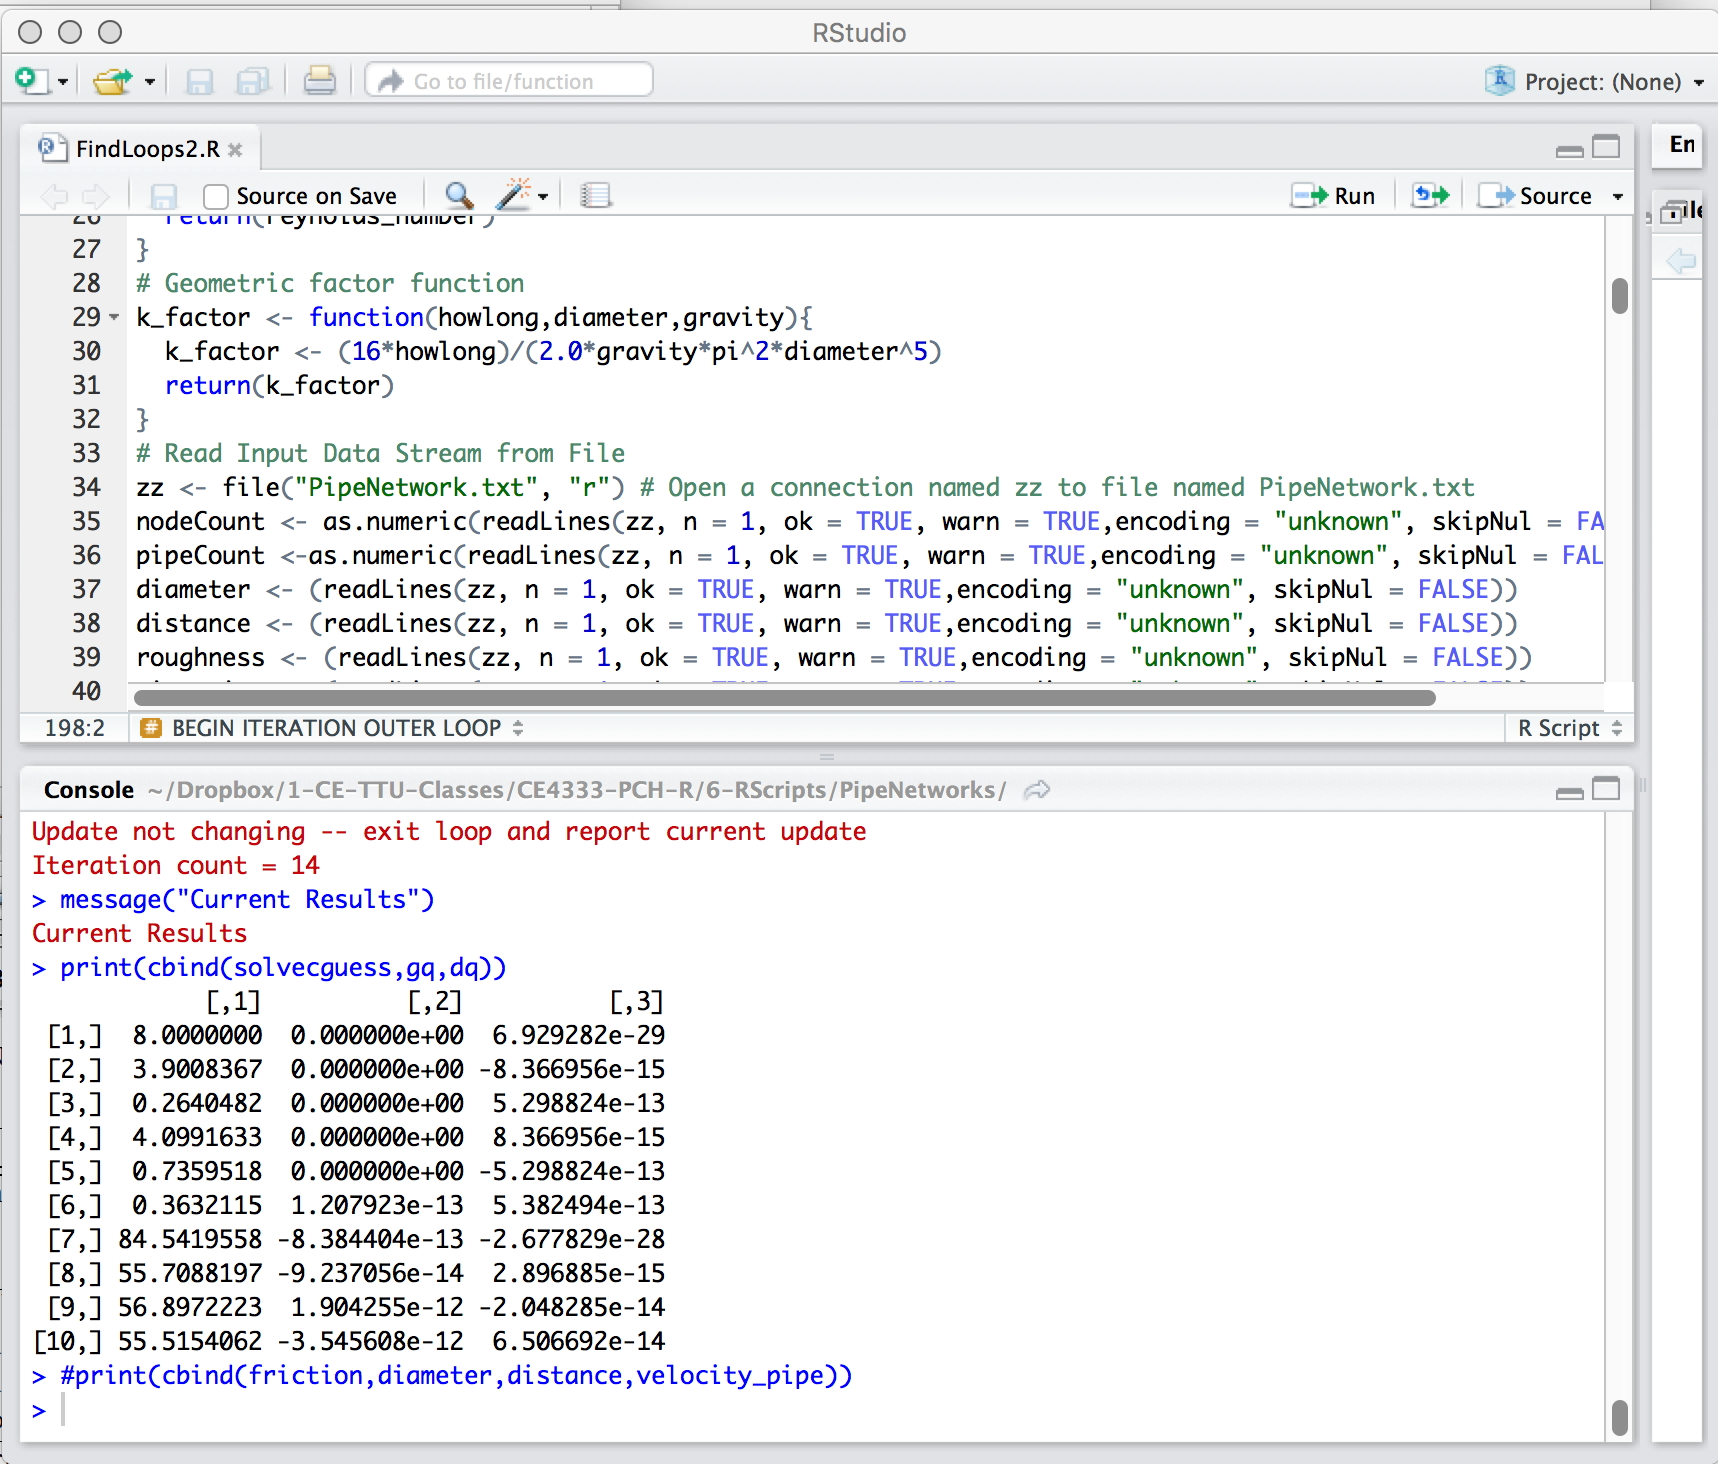
\includegraphics[width=6in]{./9-PipelineNetworkAnalysis/FindLoopsRun.jpg}
%   \caption{Screen capture of \textbf{R} script for pipe network analysis}
%   \label{fig:FindLoopsRun} 
%\end{figure}
%
%%%%%%%%%%%%%%%%%%%%%%%%%%%%%%%%%%%%%%%
%%%%%%%%%%%%%%%%% ES8 %%%%%%%%%%%%%%%%%%%
%%%%%%%%%%%%%%%%%%%%%%%%%%%%%%%%%%%%%%%
%\clearpage
%\subsection{Exercises}
\begingroup
\begin{center}
{\textbf{{ CE 3305 Engineering Fluid Mechanics} \\ Exercise Set 17 \\ Summer 2018 -- GERMANY} }
\end{center}
\endgroup
\begingroup
~\newline
\textbf{Purpose} : Apply network hydraulics principles to compute discharges and pressures in a pipeline network. \\
\textbf{Assessment Criteria} : Completion, results plausible, format correct, \textbf{R} script shown\\~\\
\textbf{Exercises}:
\begin{enumerate}
\item Figure \ref{fig:NetworkLayout} is a five-pipe network with a water supply source at Node 1, and demands at Nodes 1-5.
Table \ref{tab:PipeData} is a listing of the node and pipe data.

\begin{figure}[h!] %  figure placement: here, top, bottom, or page
\centering
   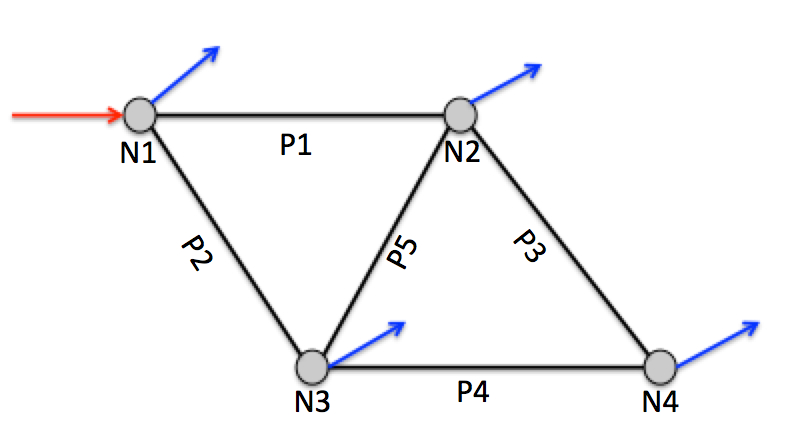
\includegraphics[width=3in]{./8-PipeNetworkHydraulics/NetworkLayout.jpg}
   \caption{Layout of Simple Network}
   \label{fig:NetworkLayout} 
\end{figure}

% Requires the booktabs if the memoir class is not being used
\begin{table}[htbp]
   \centering
   \caption{Node and Pipe Data}
    \begin{tabular}{p{1in} p{1in} p{1in} p{1in} } % Column formatting, @{} suppresses leading/trailing space
    \hline
    \hline
Pipe ID & Diameter (inches) & Length (feet) & Rougnhess (feet) \\
\hline
P1 & 8 & 800 & 0.00001  \\
P2 & 8 & 700 & 0.00001  \\
P3 & 8 & 700 & 0.00001  \\
P4 & 8 & 800 & 0.00001  \\
P5 & 6 & 600 & 0.00001  \\
\hline
\hline
Node ID & Demand (CFS) & Elevation (feet) & Head (feet) \\
\hline
N1 & 2.0 & 0.0 & 100 \\
N2 & 4.0 & 0.0 & ~? \\
N3 & 3.0 & 0.0 & ~? \\
N4 & 1.0 & 0.0 & ~? \\
   \end{tabular}
   \label{tab:PipeData}
\end{table}

Code the script, build an input file, and determine the flow distribution
In your solution you are to supply
\begin{enumerate}
\item An analysis showing the development of the node-arc incidence matrix based on the flow directions in Figure \ref{fig:NetworkLayout},
\item The input file you constructed to provide the simulation values to your script, and
\item A screen capture (or output file) showing the results.
\end{enumerate}


\item Code the script and determine the flow distribution in Figures \ref{fig:pipe-net} and \ref{fig:pipe-net-loops}.  Assume Node N1 has a total head of 300 feet. 

\begin{figure}[h!] %  figure placement: here, top, bottom, or page
   \centering
   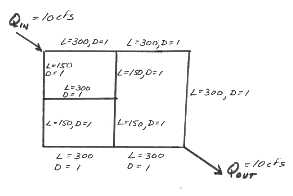
\includegraphics[width=3in]{./8-PipeNetworkHydraulics/pipe-net.jpg} 
   \caption{Pipe network for illustrative example with supply and demands identified.  Pipe lengths (in feet) and diameters (in feet) are also depicted.}
   \label{fig:pipe-net}
\end{figure}

\begin{figure}[h!] %  figure placement: here, top, bottom, or page
   \centering
   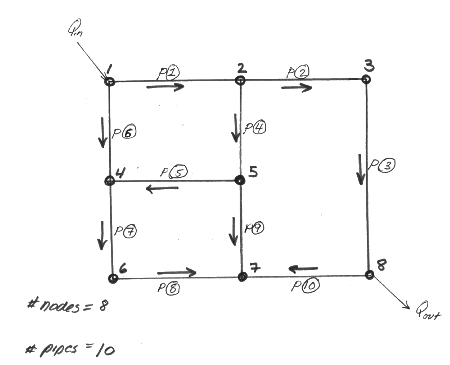
\includegraphics[width=3in]{./8-PipeNetworkHydraulics/pipe-net-loops.jpg} 
   \caption{Pipe network for illustrative example with pipes and nodes labeled.}
   \label{fig:pipe-net-loops}
\end{figure}

In your solution you are to supply
\begin{enumerate}
\item An analysis showing the development of the node-arc incidence matrix based on the flow directions in Figure \ref{fig:pipe-net-loops},
\item The input file you constructed to provide the simulation values to your script, and
\item A screen capture (or output file) showing the results.
\end{enumerate}

\item Modify the script to include node elevation information to compute pressures.  Assume all nodes are at elevation 200 feet.

\end{enumerate}
